% Paper Template; see https://github.com/author-kit

\documentclass[10pt,twocolumn,letterpaper]{article}
\usepackage{amsmath,amssymb}
\usepackage{graphicx} % for \includegraphics
\usepackage{CJKutf8}  % Chinese under pdfLaTeX

% NOTE: The AAAI 2027 style requires pdfLaTeX; avoid XeLaTeX-only packages (e.g., ctex).

% Custom commands (mirrored from main.tex so the standalone appendix compiles)
\newcommand{\ours}{BlackHoleMerge}
\newcommand{\eg}{\emph{e.g.} }
\newcommand{\ie}{\emph{i.e.} }
\newcommand{\cf}{\emph{cf.} }
\newcommand{\etc}{\emph{etc.} }

% Tables / layout
\usepackage{array}
\usepackage{booktabs}
\usepackage{multirow}
\usepackage{makecell}
\usepackage{float}
\usepackage{pifont}

% Colors + hyperlinks
\usepackage[table]{xcolor}
\definecolor{customblue}{rgb}{0.21,0.49,0.74}
\definecolor{customblue2}{rgb}{0.21,0.49,0.74}
\definecolor{lightpink}{RGB}{255, 182, 193}
\usepackage[pagebackref,breaklinks,colorlinks,allcolors=customblue]{hyperref}

%%%%%%%%% PAPER TYPE - PLEASE UPDATE FOR FINAL VERSION

% Import additional packages in the preamble file, before hyperref

% It is strongly recommended to use hyperref, especially for the review version.
% hyperref with option pagebackref eases the reviewers' job.
% Please disable hyperref *only* if you encounter grave issues,
% e.g. with the file validation for the camera-ready version.
%
% If you comment hyperref and then uncomment it, you should delete *.aux before re-running LaTeX.
% (Or just hit 'q' on the first LaTeX run, let it finish, and you should be clear).



% \bibliographystyle{unsrtnat}

%%%%%%%%% PAPER ID - PLEASE UPDATE
\def\paperID{****} % *** Enter the Paper ID here
\def\confName{DocumentParsing}
\def\confYear{2026}

%%%%%%%%% TITLE - PLEASE UPDATE
\title{Boosting Document Parsing Efficiency and Performance \\ with Coarse-to-Fine Visual Processing}

%%%%%%%%% AUTHORS - PLEASE UPDATE

\begin{document}
\begin{CJK}{UTF8}{gbsn}


% \maketitle

% \begin{abstract}
High-resolution document VLMs typically encode thousands of visual tokens per page, yet the content of a document page is highly non-uniform: text, formulas, and tables carry most of the semantic information, while blank margins and background regions occupy large portions of the page. Existing compression strategies---fixed downsampling, token pruning, and fixed-ratio merging---either overlook this density heterogeneity or discard tokens outright, making it hard to reach high compression rates without degrading fine-grained OCR performance. We propose BlackHoleMerge, a training-based, content-adaptive method for visual-token compression in document VLMs. Our approach stems from a simple observation: a pretrained document VLM already embeds an annotation-free density signal within its own internal representations---the L2 norm of its ViT Key (K) vectors---which reflects the text and structural density of each page region. BlackHoleMerge translates this intrinsic signal directly into compression decisions inside the visual encoder. It preserves text- and structure-dense regions at fine granularity, while folding blank and redundant regions into these informative tokens so that information is compressed rather than discarded. We then train the model to adapt to the resulting shortened visual sequences. As a result, the model dynamically reallocates its visual budget according to document density; requiring neither external detectors nor predefined compression ratios, our scheme performs compression in a fully adaptive manner. We validate BlackHoleMerge on multiple end-to-end OCR backbones. On OmniDocBench v1.6, it achieves over 70\% average visual-token compression while maintaining nearly lossless parsing accuracy relative to the uncompressed models. These results demonstrate that content-adaptive token compression is an effective route to improving the efficiency of end-to-end document VLMs.11
\end{abstract}    
% \section{Introduction}
\label{sec:intro}

Human readers do not process a document page uniformly or strictly in layout order. Under a limited attention budget, they first focus on regions that carry the most information, such as text, formulas, tables, and structural boundaries, while assigning lower priority to blank margins, line spacing, paper texture, and background areas. Importantly, these low-priority cues are not discarded entirely; they are compressed into coarser contextual representations. This ``rank first, compress later'' behavior allows humans to read complex pages efficiently with limited cognitive resources.

End-to-end document VLMs simplify traditional OCR pipelines by directly mapping a full page image to structured OCR outputs, avoiding the coupling among detection, recognition, and reconstruction modules. However, this simplification shifts the computational burden to visual token sequences. A high-resolution page often produces thousands of visual tokens, many of which come from blank margins and low-information backgrounds, yet consume the same ViT and LLM computation as tokens corresponding to text, formulas, and tables. This uniform processing is mismatched with the highly non-uniform information distribution of document pages.

\begin{figure}[t]
\centering
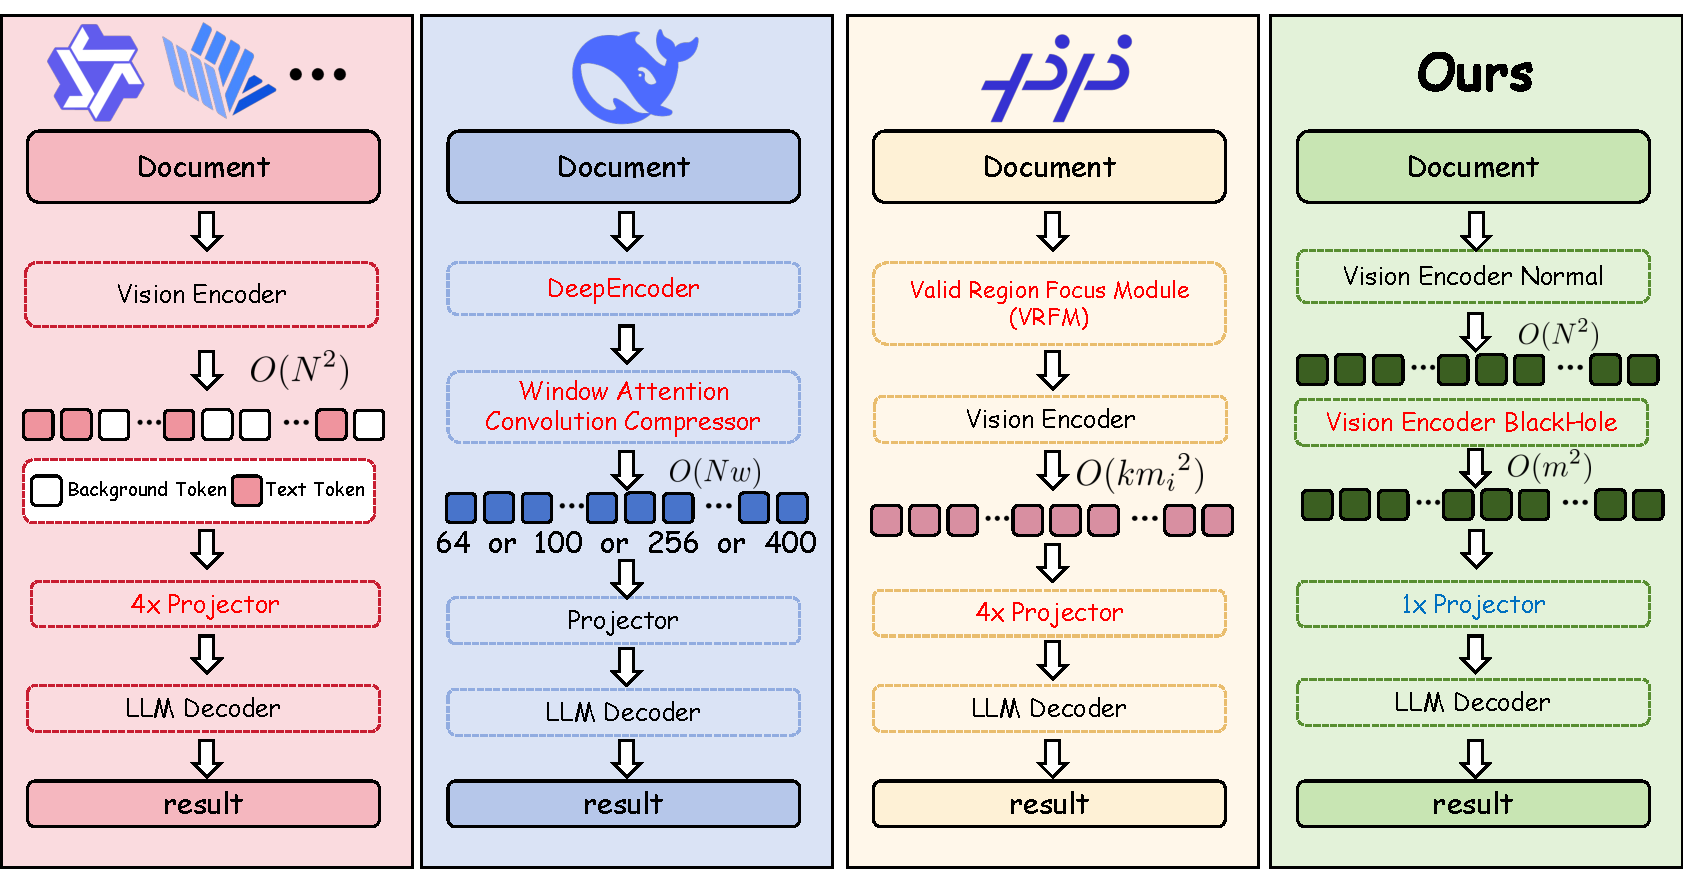
\includegraphics[width=\linewidth]{figures/final/compare_model.pdf}
\caption{Comparison between existing document parsing pipelines and \ours{}. Unlike fixed compression or external region selection, \ours{} reallocates the visual token budget inside the ViT according to document content density.}
\end{figure}

Existing compression methods do not fully resolve this mismatch. Fixed projectors or downsampling cannot distinguish text-dense regions from blank areas. Token pruning shortens the sequence, but directly removes discarded information. Token merging preserves more information than pruning, but usually relies on fixed ratios or global thresholds and therefore cannot adapt its compression strength to each page. Multi-stage OCR systems can crop redundant regions with external layout modules, but they change the setting of end-to-end VLMs and introduce additional detectors. This leads to a key question: without introducing an external detector, can an end-to-end document VLM infer from its own representations which visual tokens should be preserved first and which information can be compressed?

Our answer is yes. We find that the L2 norm of ViT Key vectors in pretrained document VLMs provides an annotation-free signal of content density. Across multiple OCR/document VLMs, text and structured content regions usually have higher K-norms, while background regions have lower K-norms. Based on this observation, we propose \ours{}, a content-adaptive visual token merging method for end-to-end document VLMs. At an intermediate ViT layer, \ours{} converts K-norms into density scores, keeps high-density tokens as local representatives, and merges low-density tokens into retained tokens according to K-vector similarity. In this way, important content is preserved first, while secondary content is compressed rather than hard-pruned, avoiding the information loss of pruning and the content-independent schedule of fixed merging.

To obtain stable compression decisions, \ours{} further uses merge-aware supervised fine-tuning to adapt the model to merged visual representations, and lightweight reinforcement learning to learn sharper keep/merge boundaries under quality constraints. We validate \ours{} on multiple end-to-end document VLM settings. Experiments show that it substantially reduces visual tokens with nearly lossless parsing accuracy, achieving over 70\% average visual token compression on OmniDocBench v1.6.
% \input{sec/2_formatting}
% \input{sec/3_finalcopy}
% {
%     \small
%     \bibliographystyle{ieeenat_fullname}
%     \bibliography{main}
% }

% WARNING: do not forget to delete the supplementary pages from your submission 
\clearpage
\setcounter{page}{1}
\setcounter{section}{0}
\setcounter{table}{0}
\setcounter{figure}{0}
% \setcounter{footnote}{0}
\renewcommand{\thesection}{\Roman{section}}
\renewcommand{\thetable}{S\arabic{table}}
\renewcommand{\thefigure}{S\arabic{figure}}

\section{Theoretical Analysis of Token Compression}
\label{sec:supp_derivation}

This section provides a rigorous analysis of the proposed token-compression
framework (instantiated as \ours{}), covering its
\emph{structural integrity}, \emph{ranking-adaptation mechanism}, and
\emph{computational savings}. The argument proceeds as follows:
(I.A) defines the K-norm density and the token-selection rule and shows the
criterion is \emph{relative}; (I.B) shows the absorption assignment is a
complete, disjoint partition with a bounded local perturbation; (I.C) explains
how, in the CE-only SFT stage, gradients \emph{indirectly} reshape the K-norm
ranking; (I.D) derives first-order conditions for rank swaps and for crossing the
keep/absorb threshold; (I.E) analyzes the non-differentiability of hard
compression and how it dictates the division of labor across training stages;
and (I.F) quantifies the complexity reduction from mid-layer compression.
We stress that the following propositions establish \emph{structural} results
(non-emptiness, complete assignment, re-ranking conditions, and a local
perturbation bound); preserving downstream OCR/parsing accuracy is an
\emph{empirical} claim, validated by the training and evaluation results in the
main paper.

\subsection{K-norm Density and Token Selection}

The core of \ours{} is a \emph{per-image, relative} density criterion: whether a
token is retained depends on its K-norm \emph{relative to the other tokens of the
same image}, not on its absolute magnitude. We first define it and then prove
this relative property.

Let $\{x_i\}_{i=1}^{N}$ with $x_i\in\mathbb{R}^{d_x}$ be the input tokens of the
$\ell$-th visual Transformer layer, with attention keys and their norms
\begin{equation}
    k_i=W_Kx_i+b_K\in\mathbb{R}^{d_k},\qquad
    r_i=\lVert k_i\rVert_2 .
    \label{eq:key_norm}
\end{equation}
Over the $N$ tokens of one image, we compute the mean and standard deviation of
the K-norms
\begin{equation}
    \mu=\frac{1}{N}\sum_{t=1}^{N}r_t,\qquad
    \sigma=\sqrt{\frac{1}{N}\sum_{t=1}^{N}(r_t-\mu)^2},
    \label{eq:key_statistics}
\end{equation}
and turn them into a density via z-score normalization followed by a sigmoid,
\begin{equation}
    z_i=\frac{r_i-\mu}{\sigma+\epsilon},\qquad
    d_i=\operatorname{sigmoid}(z_i)\in(0,1).
    \label{eq:density}
\end{equation}
Let $S=\{i\mid d_i\ge 1/2\}$ be the retained absorber set and
$R=\{1,\dots,N\}\setminus S$ the set to be absorbed. Since the sigmoid is
monotone and $\operatorname{sigmoid}(0)=1/2$, the keep criterion is equivalent to
``K-norm above the image mean'':
\begin{equation}
    d_i\ge\tfrac12
    \;\Longleftrightarrow\; z_i\ge0
    \;\Longleftrightarrow\; r_i\ge\mu .
    \label{eq:threshold_equivalence}
\end{equation}
Hence the threshold $0.5$ is not a hyper-parameter to tune, but the natural
boundary set by the per-image average density.

\paragraph{The criterion is relative (a zero-sum competition).}
Summing \eqref{eq:density} over the image and using $\sum_i(r_i-\mu)=0$ yields
\begin{equation}
    \sum_{i=1}^{N}z_i
    =\frac{1}{\sigma+\epsilon}\sum_{i=1}^{N}(r_i-\mu)=0 .
    \label{eq:zscore_sum_zero}
\end{equation}
Equation~\eqref{eq:zscore_sum_zero} shows the z-scores always sum to zero: if any
token has $z_i>0$, some other token must have $z_j<0$. Two consequences follow.
\emph{(i) Relativity.} The keep/absorb partition reflects each token's rank
\emph{relative to the image mean}, not its absolute K-norm; when one token's
density rises and its rank moves up, another token's rank must move down.
\emph{(ii) Scale invariance.} If all $r_i$ undergo the same positive affine map
$r_i\mapsto ar_i+b\ (a>0)$, then $\mu$ and $\sigma$ scale accordingly, $z_i$ is
unchanged, and so is the partition $S/R$. Together these imply that
\textbf{any effective change to the compression partition cannot come from a
uniform rescaling of all tokens, but must arise from \emph{non-uniform} per-token
updates of the K-norms.} This is exactly what I.C addresses: how training
produces such non-uniform updates—and thereby re-ranks the density—when the only
supervision is CE and the hard selection is non-differentiable.

\subsection{K-space Assignment and Structural Integrity}

This subsection establishes two structural properties of the absorption
assignment—\emph{the retained set is non-empty} (an absorber always exists) and
\emph{every absorbee is assigned uniquely} (no token is dropped or double
counted)—so that compression neither loses nor duplicates any token. We then
bound the local perturbation induced by the merge.

\paragraph{The retained set is non-empty.}
Since $r_{\max}=\max_i r_i\ge\mu$ (the maximum is at least the mean) and by
\eqref{eq:threshold_equivalence}, the token attaining the largest K-norm
satisfies $d_i\ge 1/2$; hence
\begin{equation}
    S=\{i\mid d_i\ge 1/2\}\neq\varnothing .
\end{equation}
This guarantees that the $\arg\max_{i\in S}$ below is always taken over a
non-empty set, so the assignment is well defined.

\paragraph{Completeness and disjointness of the assignment.}
For each absorbee $j\in R$, its absorber is chosen by density-weighted cosine
similarity of the Key vectors:
\begin{equation}
    a(j)=\arg\max_{i\in S}
    \left[\frac{k_j^\top k_i}{\lVert k_j\rVert_2\,\lVert k_i\rVert_2}\,d_i\right].
    \label{eq:assignment}
\end{equation}
The cosine term measures feature compatibility, while $d_i$ favors reliable
high-density absorbers. Aggregating all assignments is equivalent to maximizing
\begin{equation}
    \max_{a:R\rightarrow S}\;\sum_{j\in R}
    \operatorname{cos}(k_j,k_{a(j)})\,d_{a(j)} .
    \label{eq:assignment_objective}
\end{equation}
The key observation is that \eqref{eq:assignment_objective} is \emph{fully
separable} over $j$: the choice of absorber for one $j$ does not affect the term
of any other $j$. Therefore the mapping obtained by an independent per-token
$\arg\max$ (i.e., \eqref{eq:assignment}) is the global optimum of this objective,
with no combinatorial search required. Moreover, since $\arg\max$ returns a
unique absorber for each $j$, the family
$\{\,\{j\in R:a(j)=i\}\,\}_{i\in S}$ forms a disjoint partition of $R$: every
absorbee belongs to exactly one absorber, with neither missing nor duplicated
assignments. This is the precise meaning of ``complete assignment'' for the
compression operator.

\paragraph{The merge has a bounded local perturbation.}
Let $h_i\in\mathbb{R}^{d}$ be the visual feature passed to the downstream
projector/LLM. Each absorber $i\in S$ absorbs its assigned tokens through a
density-weighted residual:
\begin{equation}
    \widetilde h_i=h_i+
    \sum_{j\in R:\,a(j)=i}d_j\,(h_j-h_i),\qquad i\in S.
    \label{eq:residual_merge}
\end{equation}
Note this \emph{pulls} the absorber toward its absorbees in a weighted manner,
rather than taking a plain average. By the triangle inequality, the change of
each absorber feature satisfies
\begin{equation}
    \bigl\lVert\widetilde h_i-h_i\bigr\rVert_2
    \le\sum_{j\in R:\,a(j)=i}d_j\,\bigl\lVert h_j-h_i\bigr\rVert_2 .
    \label{eq:local_bound}
\end{equation}
Equation~\eqref{eq:local_bound} shows the perturbation is \emph{doubly}
suppressed: low-density tokens carry a small weight $d_j$, explicitly attenuating
their influence, while \eqref{eq:assignment} tends to assign $j$ to an absorber
close to it in K-space, keeping the residual distance
$\lVert h_j-h_i\rVert$ small as well.

We note honestly that \eqref{eq:residual_merge} is a density-weighted residual
and does \emph{not} conserve the unweighted feature sum $\sum_i h_i$. Hence our
rigorous claim is that the ``density-weighted residual is controlled,'' not that ``visual features are exactly conserved.''

\subsection{How CE Indirectly Drives the K-norm Ranking}

\paragraph{The core question.}
The keep/absorb decision of \ours{} relies on a hard threshold and a hard
$\arg\max$ assignment, both non-differentiable. Why, then, does the K-norm
ranking change at all during an SFT stage that uses \emph{only} teacher-forcing
cross-entropy (CE)? The answer is that CE does \emph{not} differentiate the
density directly; instead, it first alters the attention Key representations, and
the resulting change in Key norms reshapes the K-norm ranking. The full indirect
chain is
\begin{equation}
    \mathcal{L}_{\mathrm{CE}}
    \longrightarrow \text{attention logits}
    \longrightarrow k_i
    \longrightarrow r_i=\lVert k_i\rVert_2
    \longrightarrow z_i
    \longrightarrow \text{keep/absorb decision}.
    \label{eq:ce_ranking_chain}
\end{equation}
Following this chain, we first derive the CE gradient w.r.t.\ a single Key vector
(in three steps), and then convert it, through the shared projection parameters,
into a change of the K-norm.
\paragraph{Notation.}
Let $a$ index the query token and $b$ the candidate key/value token; let
$q_a,k_b,v_b$ be the query, key, and value at positions $a,b$ in the attention
head, $s_{ab}$ the attention logit of $a$ over $b$, $\alpha_{ab}$ the softmax
weight, and $y_a$ the attention output. Write
$g_a=\partial\mathcal{L}_{\mathrm{CE}}/\partial y_a$ for the gradient
back-propagated from the downstream projector, LLM, and CE to this attention
output. A single head satisfies
\begin{equation}
    s_{ab}=\frac{q_a^\top k_b}{\sqrt d},\qquad
    \alpha_{ab}=\frac{\exp(s_{ab})}{\sum_c\exp(s_{ac})},\qquad
    y_a=\sum_b\alpha_{ab}v_b.
    \label{eq:attention}
\end{equation}

\paragraph{Step 1: gradient w.r.t.\ the attention weights.}
Since $y_a=\sum_b\alpha_{ab}v_b$ gives $\partial y_a/\partial\alpha_{ab}=v_b$,
\begin{equation}
    \frac{\partial\mathcal{L}_{\mathrm{CE}}}{\partial\alpha_{ab}}
    =\Bigl(\frac{\partial\mathcal{L}_{\mathrm{CE}}}{\partial y_a}\Bigr)^{\!\top}
    \frac{\partial y_a}{\partial\alpha_{ab}}
    =g_a^\top v_b.
    \label{eq:ce_to_attention_weight}
\end{equation}

\paragraph{Step 2: gradient w.r.t.\ the attention logits.}
Softmax maps a set of scores $\{s_{ac}\}_c$ to normalized weights
$\{\alpha_{ac}\}_c$; perturbing any $s_{ab}$ changes all $\alpha_{ac}$, with
Jacobian
\begin{equation}
    \frac{\partial\alpha_{ac}}{\partial s_{ab}}
    =\alpha_{ac}\bigl(\mathbb{I}[b=c]-\alpha_{ab}\bigr),
    \label{eq:softmax_jacobian}
\end{equation}
where $\mathbb{I}[\cdot]$ is the indicator and $c$ ranges over all output weights.
By the multivariate chain rule, substituting
\eqref{eq:ce_to_attention_weight}--\eqref{eq:softmax_jacobian} and summing over
$c$ with $\sum_c\alpha_{ac}v_c=y_a$ gives
\begin{equation}
    \frac{\partial\mathcal{L}_{\mathrm{CE}}}{\partial s_{ab}}
    =\sum_c\frac{\partial\mathcal{L}_{\mathrm{CE}}}{\partial\alpha_{ac}}
    \frac{\partial\alpha_{ac}}{\partial s_{ab}}
    =\alpha_{ab}\,g_a^\top(v_b-y_a).
    \label{eq:ce_to_logit}
\end{equation}
\paragraph{Step 3: gradient w.r.t.\ the Key vector.}
The Key $k_b$ influences the loss only through the logits $\{s_{ab}\}_a$ in which
it participates, and $\partial s_{ab}/\partial k_b=q_a/\sqrt d$. Summing over all
query indices $a$,
\begin{equation}
    \frac{\partial\mathcal{L}_{\mathrm{CE}}}{\partial k_b}
    =\sum_a\frac{\partial\mathcal{L}_{\mathrm{CE}}}{\partial s_{ab}}
    \frac{\partial s_{ab}}{\partial k_b}
    =\frac{1}{\sqrt d}\sum_a
    \alpha_{ab}\,\bigl[g_a^\top(v_b-y_a)\bigr]\,q_a.
    \label{eq:ce_to_key}
\end{equation}
Equation~\eqref{eq:ce_to_key} shows that as long as token $b$ contributes to some
query's attention and can affect the downstream output, CE generally sends a
non-zero gradient back to its Key. Because $\alpha_{ab},v_b,q_a,g_a$ differ across
visual tokens, each token's Key-update direction is different; this
\emph{heterogeneous} gradient is the root cause of K-norm re-ranking during
training.

\paragraph{From Key gradients to K-norm changes.}
Write $g_i^K=\partial\mathcal{L}_{\mathrm{CE}}/\partial k_i$. Crucially, all visual
tokens \emph{share} the same Key-projection parameters $(W_K,b_K)$, so the $k_i$
are not independent variables: the gradient of any token couples, through the
shared parameters, into every other token. The standard SGD update is
\begin{equation}
    W_K^+=W_K-\eta\sum_{t=1}^{N}g_t^K x_t^\top,\qquad
    b_K^+=b_K-\eta\sum_{t=1}^{N}g_t^K,
    \label{eq:sgd_wk}
\end{equation}
with learning rate $\eta$ and $N$ tokens per image. Substituting into
$k_i^+=W_K^+x_i+b_K^+$ yields the first-order Key change of token $i$ within one
step,
\begin{equation}
    k_i^+-k_i=-\eta\,G_i^K,\qquad
    G_i^K=\sum_{t=1}^{N}g_t^K\bigl(x_t^\top x_i+1\bigr).
    \label{eq:induced_key_update}
\end{equation}
The coupling term $G_i^K$ means: the gradients $g_t^K$ of all tokens in the image
combine—through the shared parameters, weighted by $(x_t^\top x_i+1)$ (with
$x_t^\top x_i$ from $W_K$ and the constant $1$ from the bias $b_K$)—to determine
the effective update direction of token $i$.

Let $u_i=k_i/\lVert k_i\rVert_2$ be the unit radial vector. A first-order Taylor
expansion of $r_i=\lVert k_i\rVert_2$ at $k_i$, using
\eqref{eq:induced_key_update} and dropping $O(\eta^2)$, gives
\begin{equation}
    r_i^+-r_i=-\eta\,u_i^\top G_i^K+O(\eta^2).
    \label{eq:norm_update}
\end{equation}
Thus the K-norm rises or falls solely according to the projection of the coupled
gradient $G_i^K$ onto the current Key direction $u_i$: $r_i$ increases when
$u_i^\top G_i^K<0$ and decreases when $u_i^\top G_i^K>0$.

\paragraph{Summary.}
By \eqref{eq:zscore_sum_zero} the z-scores sum to zero, so their changes also sum to zero. Whenever the step's updates are \emph{non-uniform} across tokens (guaranteed by the heterogeneous gradient of \eqref{eq:ce_to_key}), the image
must contain tokens whose relative density rises and others whose relative
density falls—setting up a K-norm rank swap and a keep/absorb mask switch at the
next forward pass. I.D makes this precise as a first-order flip condition.

\subsection{First-order Conditions for Rank Swaps and Threshold Crossings}

I.C showed that CE induces \emph{heterogeneous} radial updates across tokens.
Building on this, we give two decidable first-order conditions: when two tokens
\emph{swap} their K-norm rank, and when a single token \emph{crosses} the
keep/absorb threshold. For brevity, denote the \emph{radial update} of token $i$
\begin{equation}
    \rho_i \;:=\; u_i^\top G_i^K,
\end{equation}
so that \eqref{eq:norm_update} reads $r_i^+-r_i=-\eta\,\rho_i+O(\eta^2)$: the
K-norm grows when $\rho_i<0$ and shrinks when $\rho_i>0$.

\paragraph{Rank swap between two tokens.}
Assume $r_i>r_j$ and define the ranking margin $m_{ij}=r_i-r_j>0$. Substituting
\eqref{eq:norm_update} for $r_i$ and $r_j$ and taking the difference gives the
updated margin
\begin{equation}
    m_{ij}^+=m_{ij}-\eta\,(\rho_i-\rho_j)+O(\eta^2).
    \label{eq:rank_margin}
\end{equation}
To first order, $j$ overtakes $i$ (i.e., $m_{ij}^+<0$) iff
\begin{equation}
    \eta\,(\rho_i-\rho_j)\;>\;m_{ij}.
    \label{eq:rank_crossing}
\end{equation}
That is, the two K-norms swap once the difference of their radial updates (times
the learning rate) offsets the original norm gap—equivalently, $j$'s norm grows
more than $i$'s by at least $m_{ij}$.

\paragraph{Threshold crossing of a single token.}
To avoid clashing with the density $d_i$, we denote the \emph{threshold margin}
\begin{equation}
    \delta_i \;:=\; r_i-\mu,
\end{equation}
where $\delta_i>0$ means retained and $\delta_i<0$ means absorbed. The image mean
updates by $\Delta\mu=\frac1N\sum_t(r_t^+-r_t)=-\eta\,\bar\rho+O(\eta^2)$ with
$\bar\rho=\frac1N\sum_t\rho_t$ the image-average radial update. Hence
\begin{equation}
    \delta_i^+-\delta_i
    =-\eta\bigl(\rho_i-\bar\rho\bigr)+O(\eta^2).
    \label{eq:threshold_margin}
\end{equation}
If a token is currently absorbed ($\delta_i<0$), a first-order sufficient
condition for it to become retained ($\delta_i^+>0$) is
\begin{equation}
    \eta\bigl(\rho_i-\bar\rho\bigr)\;<\;\delta_i\;(<0).
    \label{eq:threshold_crossing}
\end{equation}
Since $\delta_i<0$, this implies $\rho_i<\bar\rho$: only a token whose K-norm
grows \emph{faster than the image average}, by an amount (times $\eta$) large
enough to fill its current negative margin $\delta_i$, sees its relative density
rise above the mean and cross from the absorbed side to the retained side.

Combining \eqref{eq:rank_crossing} and \eqref{eq:threshold_crossing}: CE cannot
edit the discrete mask directly, but as long as the radial updates it induces are
sufficiently \emph{non-uniform} across tokens, they trigger a rank swap or a
threshold crossing at the next forward pass, thereby \emph{indirectly} reshaping
the keep/absorb partition. This closes the question raised at the start of I.C.

\subsection{Non-differentiability of Hard Compression and the Division of Labor Across Three Stages}

The deployed \ours{} contains three discrete operations that block gradient flow:
hard thresholding, $\arg\max$ hard assignment, and the stop-gradient applied to the
density weights of absorbed tokens (see Eq.~(6) in the main text). Let $d_i$ denote the
density score of a token. Within a local region that does not cross the keep/absorb
boundary, the merged output $\widetilde H$ is piecewise constant in the densities, and the
weighting term is severed by the stop-gradient; hence the gradient of the merge branch
with respect to any density is identically zero:
\begin{equation}
    \frac{\partial\widetilde H}{\partial d_i}\bigg|_{\mathrm{merge\ branch}}=0
    \;\Longrightarrow\;
    \frac{\partial\mathcal{L}_{\mathrm{CE}}}{\partial d_i}\bigg|_{\mathrm{merge\ branch}}=0 .
    \label{eq:hard_merge_gradient}
\end{equation}
Eq.~\eqref{eq:hard_merge_gradient} shows that CE cannot directly push a token's density
above the threshold through the compression operator. Its only adaptation channel is the
native visual-attention Key path derived in I.C (which can only continuously reshape the
Key representations), and the discrete mask of the next forward pass switches only when a
parameter update satisfies Eq.~\eqref{eq:rank_crossing} or
Eq.~\eqref{eq:threshold_crossing}.

This non-differentiable structure naturally dictates the division of labor across the
\textbf{three training stages}:

\textbf{Stage 1: Merge-aware SFT.} The full model is trained end-to-end with CE only.
Through the native Key path of Eq.~\eqref{eq:ce_to_key}, document-relevant tokens are
gradually re-ranked toward the absorber side, forming a \emph{coarse} density ordering
that establishes the base parsing performance; this stage characterizes the boundary
(near $0.5$) only weakly.

\textbf{Stage 2: Lightweight RL (GRPO).} We freeze the ViT, projector, and LLM, and train
only the lightweight policy MLP. Acting as a differentiable policy head, it directly
optimizes the \emph{discrete} keep/drop decision, bypassing the zero-gradient obstacle of
Eq.~\eqref{eq:hard_merge_gradient}, and tightens the compression boundary on top of the SFT
ordering to raise the compression ratio under a quality constraint.

\textbf{Stage 3: Post-SFT re-adaptation.} RL substantially shifts the distribution of
retained tokens (more aggressive compression, shorter sequences), causing an input-distribution
shift for the projector and LLM that were originally trained on the SFT distribution. To
remove this shift, we \emph{freeze the entire ViT and the policy MLP} (i.e., fix the learned
compression policy) and \emph{unfreeze only the projector and LLM}, performing a lightweight
re-adaptation for a \emph{very small number of steps} so that the downstream modules adapt to
the post-RL short visual sequence. Since the compression policy is already fixed, this stage
does not alter the keep/drop behavior; it only re-aligns the downstream representations.

Together, the three stages form a pipeline: SFT builds a task-relevant density ordering, RL
learns a more aggressive yet quality-constrained compression boundary on top of it, and
post-SFT lets the downstream projector/LLM adapt to the post-RL distribution, thereby
preserving parsing quality at a high compression ratio.

\section{Implementation and Model Adaptation}
\label{sec:supp_impl}

Because \ours{} operates on the visual-token stream \emph{inside} the encoder, it is agnostic
to the specific host VLM. To show this, we adapt it into three representative document VLMs:
PaddleOCR-VL-1.6, MinerU2-VLM, and dots.ocr. For every host we remove any external crop /
region-selection front-end and feed the full page directly into the visual encoder, so that the
measured compression is attributable to the in-encoder merge alone rather than to pipeline-level
region filtering. Where a host uses a fixed reduction projector, we adapt only the projector's
input protocol so that its placeholders match the compressed sequence, leaving the backbone
weights unchanged.

\subsection{PaddleOCR-VL-1.6}
The full PaddleOCR-VL-1.6 system is a coarse-to-fine pipeline: a layout/region module first
localizes valid regions on the full page and filters margins, blanks, and background, after which
the cropped high-resolution regions are parsed by the 0.9B VLM. Part of its redundancy removal
therefore happens \emph{before} the VLM, through an external region selector rather than
in-encoder token compression.

We isolate the 0.9B VLM and build an end-to-end setting without the external crop stage: the full
page enters the visual encoder directly, and token keep/merge is decided by the compression
module. To avoid entangling the original $4\times$ projector's fixed spatial reduction with our
method, we replace it with a $1\times$ per-token projector that maps the ViT hidden size $1152$ to
the LLM hidden size $1024$ and performs no extra $2\times2$ spatial merge. Differences across
variants are thus attributable to the training path and the token-compression policy.

\subsection{MinerU2-VLM}
MinerU2's full parser is likewise a pipeline that selects regions or page blocks by layout and
task type before the VLM parses text, formulas, and structure; again, part of the redundancy
removal happens outside the VLM. To test whether \ours{} depends on a single architecture, we
extract MinerU2's 0.9B VLM and build an end-to-end setting with no front-end region cropping: the
page enters the visual encoder directly.

MinerU2-VLM uses a 26-layer SigLIP vision tower with hidden size $1152$. Under its single-tile
input, each page is resized to one $384\times384$ tile, producing
\begin{equation}
    N_0 = 27 \times 27 = 729
\end{equation}
visual tokens, which a per-token MLP projector maps to the LLM hidden size $896$ with no extra
spatial merge; the token count is thus governed solely by \ours{}. We insert the merge head after
SigLIP layer $20$: the first $20$ blocks run on the full $729$-token sequence, layer $20$ builds
the K-norm density and selects absorbers, low-density tokens are merged into their most similar
absorber via density-weighted residuals, and the shortened sequence continues through blocks
$21$--$25$, the projector, and the LLM. Merging therefore occurs \emph{inside} the encoder, so the
self-attention of blocks $21$--$25$, the projector cost, and the LLM prefill context all shrink.

Unlike fixed-count reduction, the retained length is set adaptively by each tile's K-norm density
distribution: within one training batch the $729$ input tokens can be compressed to different
lengths (e.g., $418, 434, 456, 455, 419, 434, 412, 401$ for eight tiles). Denser text, formula, or
complex-layout pages keep more tokens, while background and low-information regions are absorbed
more strongly. For a fair comparison, the no-merge baseline and the \ours{} model share the same
MinerU2-VLM initialization, resolution, SigLIP backbone, per-token projector, and LLM; only the
adaptive merge after layer $20$ differs, so the quality/compute gap is attributable to in-encoder
merging rather than external cropping or projector changes.

\subsection{dots.ocr}
As an OCR-centric VLM, dots.ocr tightly couples text layout with visual tokens and is highly
sensitive to uniform pruning. We modify its dense feature-map projection to accept
variable-length compressed token inputs instead of a static grid, letting the merge wrap closely
around dense content blocks in multi-column layouts. The adapted version achieves a
\textbf{40.0\% token saving} without character-level information loss or layout fragmentation.

\subsection{Training and Model-Selection Details}
To aid reproducibility, Table~\ref{tab:supp_config} collects the training configuration
shared across hosts. All stages use the same corpus of roughly $9$M document pages drawn
from the public PaddleOCR data, with parsing labels auto-generated by the PaddleOCR-VL
series; the same corpus is kept across the compared settings so differences come from the
compression path rather than the data. The three stages follow the freezing schedule
described above: merge-aware SFT trains the full model, GRPO trains only the
$\sim$74K-parameter policy MLP with the ViT/projector/LLM frozen, and the short post-SFT
stage unfreezes only the projector and LLM. The merge layer per host (PaddleOCR-VL-1.6 L9,
MinerU2-VLM L20, dots.ocr L32) and the reported ``best'' configuration are chosen on a
held-out validation split disjoint from the OmniDocBench~v1.6 evaluation set, so that the
test benchmark is not used for model selection. Optimizer, learning-rate, batch-size, and
step-count entries left as ``--'' are filled with the exact values in the final version.
% TODO(核实): 确认 held-out validation split 描述属实、且与 OmniDocBench v1.6 无重叠；补齐 optimizer/LR/batch/steps/seed/分辨率 真实值。

\begin{table}[t]
\centering
\fontsize{7.6}{9}\selectfont
\setlength{\tabcolsep}{4pt}
\begin{tabular*}{\columnwidth}{@{\extracolsep{\fill}}l l@{}}
\toprule
\textbf{Item} & \textbf{Value} \\
\midrule
Training corpus & $\sim$9M public PaddleOCR pages \\
Labels & auto-generated by PaddleOCR-VL series \\
Projector (Paddle / MinerU2) & $1\times$ per-token, $1152{\to}1024$ / $1152{\to}896$ \\
Merge layer (Paddle/MinerU2/dots) & L9 / L20 / L32 \\
Policy MLP & $\sim$74K params, input full Key vector \\
GRPO rollouts $K$ & 8 \\
Stage-1 (merge-aware SFT) & full model; optimizer/LR/steps: -- \\
Stage-2 (GRPO RL) & ViT+proj+LLM frozen; LR/steps: -- \\
Stage-3 (post-SFT) & proj+LLM only; steps: -- \\
Input resolution & -- \\
Batch size / seed & -- / -- \\
Hardware & $8\times$H800 \\
\bottomrule
\end{tabular*}
\caption{Training and model-selection configuration for \ours{}. Known settings are listed
explicitly; entries marked ``--'' are exact hyper-parameters to be filled in the final
version. Configurations are selected on a validation split disjoint from OmniDocBench~v1.6.}
\label{tab:supp_config}
\end{table}

%============================================================
% C. Additional Ablation Studies
%============================================================
\section{Additional Ablation Studies}
\label{sec:supp_ablation}

\subsection{Per-Layer and Cross-Model Quality--Efficiency Ablation}
Table~\ref{tab:supp_layer_full} gives the full quality--efficiency breakdown of the
merge-layer ablation that the main text condenses. For PaddleOCR-VL-1.6 we report all
three candidate merge layers (L3/L6/L9) with both efficiency (retained tokens, ViT and
prefill TFLOPs) and the complete OmniDocBench~v1.6 parsing metrics
(Text Edit, Formula CDM, Table TEDS/TEDS\textsubscript{s}, Reading-Order Edit, and
Overall). Merging earlier (L3) removes the most ViT compute but slightly weakens parsing,
whereas a mid/late layer (L9) attains the best overall quality at a comparable token
budget, which is the configuration reported as \ours{}~(best) in the main text. For the
other two hosts we do not sweep layers but fix a single mid/late merge point consistent
with their K-norm separation profile (MinerU2-VLM after layer~20, dots.ocr after
layer~32) and report the same ablation metrics under that fixed layer.

\begin{table*}[t]
\centering
\fontsize{8}{9.6}\selectfont
\setlength{\tabcolsep}{4pt}
\renewcommand{\arraystretch}{1.15}
\begin{tabular*}{\textwidth}{@{}l@{\extracolsep{\fill}}ccccccccc@{}}
\toprule
\shortstack[l]{\textbf{Merge}\\\textbf{Layer}} &
\textbf{Merged} & \textbf{ViT} & \textbf{Prefill} &
\shortstack{\textbf{Text}\\\textbf{Edit}$\downarrow$} &
\shortstack{\textbf{Formula}\\\textbf{CDM}$\uparrow$} &
\shortstack{\textbf{Table}\\\textbf{TEDS}$\uparrow$} &
\shortstack{\textbf{Table}\\\textbf{TEDS-S}$\uparrow$} &
\shortstack{\textbf{R-order}\\\textbf{Edit}$\downarrow$} &
\textbf{Overall}$\uparrow$ \\
\midrule
\multicolumn{10}{@{}l}{\textit{PaddleOCR-VL-1.6 (0.9B), input 4954 tokens}} \\
L3 & 1511 (-69.5\%) & 2.45 & 1.46 & 0.056 & 95.08 & 87.20 & 90.41 & 0.146 & 92.23 \\
L6 & 1421 (-71.3\%) & 2.95 & 1.10 & 0.045 & 93.77 & 85.93 & 89.33 & 0.139 & 91.75 \\
L9 & 1434 (-71.1\%) & 3.54 & 1.05 & \textbf{0.049} & \textbf{95.50} & \textbf{87.62} & \textbf{91.04} & \textbf{0.138} & \textbf{92.76} \\
\midrule
\multicolumn{10}{@{}l}{\textit{MinerU2-VLM (0.9B), input 729 tokens}} \\
L20 & -- & -- & -- & -- & -- & -- & -- & -- & -- \\
\midrule
\multicolumn{10}{@{}l}{\textit{dots.ocr (1.7B), input 21510 tokens}} \\
L32 & -- & -- & -- & -- & -- & -- & -- & -- & -- \\
\bottomrule
\end{tabular*}
\caption{Full per-layer merge ablation with combined efficiency and OmniDocBench~v1.6
parsing metrics. PaddleOCR-VL-1.6 is swept over three merge layers (L3/L6/L9); the L9 row
(bold) is the \ours{}~(best) configuration reported in the main text. MinerU2-VLM and
dots.ocr use a single fixed merge layer (L20 and L32) matched to their K-norm separation
profile; entries not yet measured are left as ``--''. Merged is the retained visual-token
count (compression rate in parentheses); ViT/Prefill are TFLOPs.}
\label{tab:supp_layer_full}
\end{table*}

\subsection{Choice of Density Signal}
A natural question is whether the L2 norm of the ViT Key vector is special, or whether any
per-token importance signal would work equally well. We therefore compare the K-norm
against alternative per-token signals under the same host, merge layer, and matched
retained-token budget: the Q-norm and V-norm from the same attention block, the L2 norm of
the layer hidden state, the mean received attention, and a random score. For each signal we
report its text/blank separability (Text, Blank, and Gap, defined as in the main-text
K-norm table) and the downstream OmniDocBench~v1.6 Overall obtained when that signal drives
the keep/merge decision. Table~\ref{tab:supp_signal} and Figure~\ref{fig:supp_signal}
summarize the result: only the K-norm produces a clear, consistently positive text--blank
gap, and using it as the density signal yields the best downstream parsing; the other
signals give a much weaker or unstable separation and degrade parsing at the same budget.
This supports using the K-norm—rather than an arbitrary importance score—as the
annotation-free density signal at the core of \ours{}.

\begin{table}[t]
\centering
\fontsize{7.6}{9}\selectfont
\setlength{\tabcolsep}{4pt}
\begin{tabular*}{\columnwidth}{@{\extracolsep{\fill}}l c c c c@{}}
\toprule
\textbf{Density signal} & \textbf{Text*} & \textbf{Blank} &
\textbf{Gap}$\uparrow$ & \textbf{Overall}$\uparrow$ \\
\midrule
% TODO: 填之前统计好的真实数值；仅 K-norm 有明显正 Gap
\textbf{L2 K-norm (Ours)} & -- & -- & -- & -- \\
Q-norm            & -- & -- & -- & -- \\
V-norm            & -- & -- & -- & -- \\
Hidden-state norm & -- & -- & -- & -- \\
Mean attention    & -- & -- & -- & -- \\
Random            & -- & -- & -- & -- \\
\bottomrule
\end{tabular*}
\caption{Choice of density signal on PaddleOCR-VL-1.6 at a matched retained-token budget.
Text/Blank/Gap follow the K-norm separability definition in the main text; Overall is the
OmniDocBench~v1.6 score when each signal drives the keep/merge decision. Only the K-norm
gives a consistently positive text--blank gap and the best downstream parsing.}
\label{tab:supp_signal}
\end{table}

\begin{figure}[t]
\centering
% TODO: 替换为密度信号可分性对比图（K-norm vs Q/V/hidden/attn/random）
\fbox{\parbox[c][0.30\linewidth][c]{0.94\linewidth}{\centering\footnotesize
Placeholder: text--blank separability of candidate density signals\\
(K-norm vs.\ Q-norm, V-norm, hidden-state norm, mean attention, random).}}
\caption{Text--blank separability of candidate density signals across layers on
PaddleOCR-VL-1.6. The K-norm is the only signal with a stable positive gap.}
\label{fig:supp_signal}
\end{figure}

\subsection{Density and Keep-Ratio Analysis}
We ablate the training path on the PaddleOCR-VL-1.6 VLM under a controlled in-encoder setting:
the same 0.9B initialization, the same $1\times$ projector, and the same data and evaluation
protocol. We compare four paths. \textbf{No-merge SFT} disables \ours{} and runs ordinary SFT,
serving as the uncompressed reference and shared backbone. \textbf{Merge-aware SFT only} enables
\ours{} from the SFT stage, so the ViT, projector, and LLM jointly adapt to the compressed token
distribution. \textbf{RL only} skips merge-aware SFT and trains the lightweight policy MLP
directly, testing whether RL can learn a compression policy without a stable density-ranking
prior. \textbf{Merge-aware SFT + Confidence-Penalty RL} first learns a coarse density ranking via
SFT, then freezes the ViT, projector, and LLM and trains only the policy MLP to refine the
keep/drop boundary near $0.5$.

Tables~\ref{tab:token_density} and~\ref{tab:keep_ratio} summarize the density and keep-ratio
ablations. Merge-aware SFT enlarges the density gap between text and blank/background tokens,
showing that the model learns to assign higher density to text, formula, and structural regions
while suppressing background. RL only can lower the overall keep ratio, but without the SFT
ranking prior it removes more text tokens and parses worse than SFT only, confirming that RL
should act as a post-SFT boundary refinement rather than a standalone compression learner. After
Confidence-Penalty RL the density distribution polarizes further: background density drops sharply,
the gray zone shrinks, and the continuous SFT ordering becomes a sharper keep/drop decision. Thus
SFT forms the task-relevant density ranking and RL learns a more aggressive but quality-constrained
boundary on top of it.

\begin{table}[t]
\centering
\fontsize{7.2}{8.4}\selectfont
\setlength{\tabcolsep}{1.8pt}
\renewcommand{\arraystretch}{1.12}
\begin{tabular*}{\columnwidth}{@{\extracolsep{\fill}}%
>{\centering\arraybackslash}m{0.13\columnwidth}
>{\centering\arraybackslash}m{0.38\columnwidth}
>{\centering\arraybackslash}m{0.13\columnwidth}
>{\centering\arraybackslash}m{0.13\columnwidth}
>{\centering\arraybackslash}m{0.13\columnwidth}
@{}}
\toprule
\multicolumn{2}{c}{\textbf{Experiment}} &
\multicolumn{3}{c}{\textbf{Token Density}} \\
\cmidrule(lr){1-2}
\cmidrule(lr){3-5}
\shortstack[c]{\textbf{Merge}\\\textbf{Layer}} &
\textbf{Strategy} &
\textbf{Text*} &
\textbf{Blank} &
\textbf{Gap*} \\
\midrule
-- & Pretrained & 0.597 & 0.441 & 0.156 \\
\midrule
\multirow[c]{3}{*}{\textbf{Layer 3}}
& Merge-aware SFT & 0.642 & 0.388 & 0.254 \\
& RL only & 0.486 & 0.211 & 0.275 \\
& Merge SFT + Confidence-Penalty RL & \textbf{0.644} & \textbf{0.071} & \textbf{0.572} \\
\cmidrule(lr){2-5}
\multirow[c]{3}{*}{\textbf{Layer 6}}
& Merge-aware SFT & \textbf{0.625} & 0.355 & 0.270 \\
& RL only & 0.472 & 0.176 & 0.296 \\
& Merge SFT + Confidence-Penalty RL & 0.562 & \textbf{0.051} & \textbf{0.512} \\
\cmidrule(lr){2-5}
\multirow[c]{3}{*}{\textbf{Layer 9}}
& Merge-aware SFT & \textbf{0.617} & 0.423 & 0.194 \\
& RL only & 0.463 & 0.238 & 0.225 \\
& Merge SFT + Confidence-Penalty RL & 0.565 & \textbf{0.082} & \textbf{0.483} \\
\bottomrule
\end{tabular*}
\caption{Token density across merge layers and training stages. Text/Blank are measured on
text and blank/background regions from OmniDocBench bounding boxes; Gap $=$ Text $-$ Blank.
RL only trains the policy without merge-aware SFT and tends to suppress text density together
with background density.}
\label{tab:token_density}
\end{table}

\begin{table}[t]
\centering
\fontsize{7.2}{8.4}\selectfont
\setlength{\tabcolsep}{1.8pt}
\renewcommand{\arraystretch}{1.12}
\begin{tabular*}{\columnwidth}{@{\extracolsep{\fill}}%
>{\centering\arraybackslash}m{0.13\columnwidth}
>{\centering\arraybackslash}m{0.36\columnwidth}
>{\centering\arraybackslash}m{0.11\columnwidth}
>{\centering\arraybackslash}m{0.10\columnwidth}
>{\centering\arraybackslash}m{0.10\columnwidth}
>{\centering\arraybackslash}m{0.10\columnwidth}
@{}}
\toprule
\multicolumn{2}{c}{\textbf{Experiment}} &
\multicolumn{4}{c}{\textbf{Keep Ratio}} \\
\cmidrule(lr){1-2}
\cmidrule(lr){3-6}
\shortstack[c]{\textbf{Merge}\\\textbf{Layer}} &
\textbf{Strategy} &
\shortstack[c]{\textbf{Gray}\\\textbf{Zone}} &
\textbf{Text*} &
\textbf{Blank} &
\textbf{Overall} \\
\midrule
-- & Pretrained & 68.7\% & 77.1\% & 41.7\% & 57.0\% \\
\midrule
\multirow[c]{3}{*}{\textbf{Layer 3}}
& Merge-aware SFT & 51.7\% & 78.7\% & 23.8\% & 47.4\% \\
& RL only & 28.9\% & 41.5\% & 13.6\% & 27.9\% \\
& Merge SFT + Confidence-Penalty RL & \textbf{2.4\%} & 64.7\% & \textbf{6.9\%} & \textbf{31.8\%} \\
\cmidrule(lr){2-6}
\multirow[c]{3}{*}{\textbf{Layer 6}}
& Merge-aware SFT & 48.0\% & 79.0\% & 21.5\% & 45.8\% \\
& RL only & 25.7\% & 43.2\% & 12.8\% & 27.4\% \\
& Merge SFT + Confidence-Penalty RL & \textbf{3.5\%} & 56.3\% & \textbf{4.1\%} & \textbf{26.6\%} \\
\cmidrule(lr){2-6}
\multirow[c]{3}{*}{\textbf{Layer 9}}
& Merge-aware SFT & 61.9\% & 80.6\% & 37.0\% & 55.8\% \\
& RL only & 34.4\% & 45.8\% & 17.9\% & 31.6\% \\
& Merge SFT + Confidence-Penalty RL & \textbf{4.2\%} & 56.5\% & \textbf{6.6\%} & \textbf{28.1\%} \\
\bottomrule
\end{tabular*}
\caption{Keep ratio across merge layers and training stages. Gray Zone denotes tokens whose
density lies in the ambiguous range around the keep/drop boundary. RL only reaches a low overall
keep ratio but retains substantially fewer text tokens than merge-aware SFT, showing that RL
needs the SFT ranking prior.}
\label{tab:keep_ratio}
\end{table}

\subsection{Locality of the Merge Assignment}
Equation~(3) of the main text selects each absorbee's target absorber by a \emph{global}
$\arg\max$ of density-weighted Key cosine similarity over all absorbers, and we argue that,
because RoPE injects position into the Key vectors, the selected absorber tends to be
spatially close. Here we quantify this claim directly. For every absorbee--absorber
assignment we measure the 2-D spatial distance between the two patches (in patch units) and
report, per merge layer, the mean and median assignment distance, the fraction of
assignments that fall within an $8$-connected local neighborhood of the absorbee, and the
cross-region merge rate (assignments whose absorber lies in a different GT content region).
Table~\ref{tab:supp_locality} summarizes these statistics and
Figure~\ref{fig:supp_locality} plots the assignment-distance distribution. The assignments
concentrate at short spatial distances with a small cross-region rate, confirming that the
global similarity rule behaves as an approximately local merge in practice rather than
linking arbitrarily distant patches.

\begin{table}[t]
\centering
\fontsize{7.6}{9}\selectfont
\setlength{\tabcolsep}{4pt}
\begin{tabular*}{\columnwidth}{@{\extracolsep{\fill}}l c c c c@{}}
\toprule
\shortstack[l]{\textbf{Merge}\\\textbf{Layer}} &
\shortstack{\textbf{Mean}\\\textbf{dist.}$\downarrow$} &
\shortstack{\textbf{Median}\\\textbf{dist.}$\downarrow$} &
\shortstack{\textbf{Within}\\\textbf{$8$-nbr}$\uparrow$} &
\shortstack{\textbf{Cross-}\\\textbf{region}$\downarrow$} \\
\midrule
% TODO: 填 assignment-distance 实测统计（patch 单位 / 百分比）
L3 & -- & -- & -- & -- \\
L6 & -- & -- & -- & -- \\
L9 & -- & -- & -- & -- \\
\bottomrule
\end{tabular*}
\caption{Assignment-distance statistics for the merge assignment on PaddleOCR-VL-1.6.
Distances are in patch units; ``Within $8$-nbr'' is the fraction of absorbees assigned to an
absorber inside their $8$-connected neighborhood; ``Cross-region'' is the fraction assigned
to an absorber in a different GT content region. Short distances and a low cross-region rate
indicate an approximately local merge.}
\label{tab:supp_locality}
\end{table}

\begin{figure}[t]
\centering
% TODO: 替换为 assignment-distance 分布图（按 merge layer）
\fbox{\parbox[c][0.30\linewidth][c]{0.94\linewidth}{\centering\footnotesize
Placeholder: distribution of absorbee$\rightarrow$absorber spatial distances\\
(per merge layer, in patch units).}}
\caption{Distribution of absorbee-to-absorber spatial assignment distances on
PaddleOCR-VL-1.6. Most assignments are short-range, supporting the locality of the merge.}
\label{fig:supp_locality}
\end{figure}

\subsection{Qualitative Comparison of Compression Rules}
Figures~\ref{fig:supp_method_parse} and~\ref{fig:supp_heavy_light} visualize, under a
matched token budget on the same PaddleOCR-VL-1.6 host, why training-free rules collapse
while \ours{} preserves parsing quality (cf.\ the method-comparison table in the main
text). Figure~\ref{fig:supp_method_parse} shows the retained-token map \emph{and} the
resulting Markdown parse for each rule: ToMe-/DivPrune-/IDPrune-style operators, never
trained on compressed sequences, scatter their kept tokens across background and shred the
parse into repeated or hallucinated fragments, whereas \ours{} concentrates retained
tokens on text and structure and produces a faithful parse close to the no-merge
reference. Figure~\ref{fig:supp_heavy_light} extends the retained-token comparison to a
graphics-heavy magazine page and an advertisement page, showing that the training-free
rules keep large blocks of background while \ours{} adaptively wraps its budget around the
textual regions.

\begin{figure*}[t]
\centering
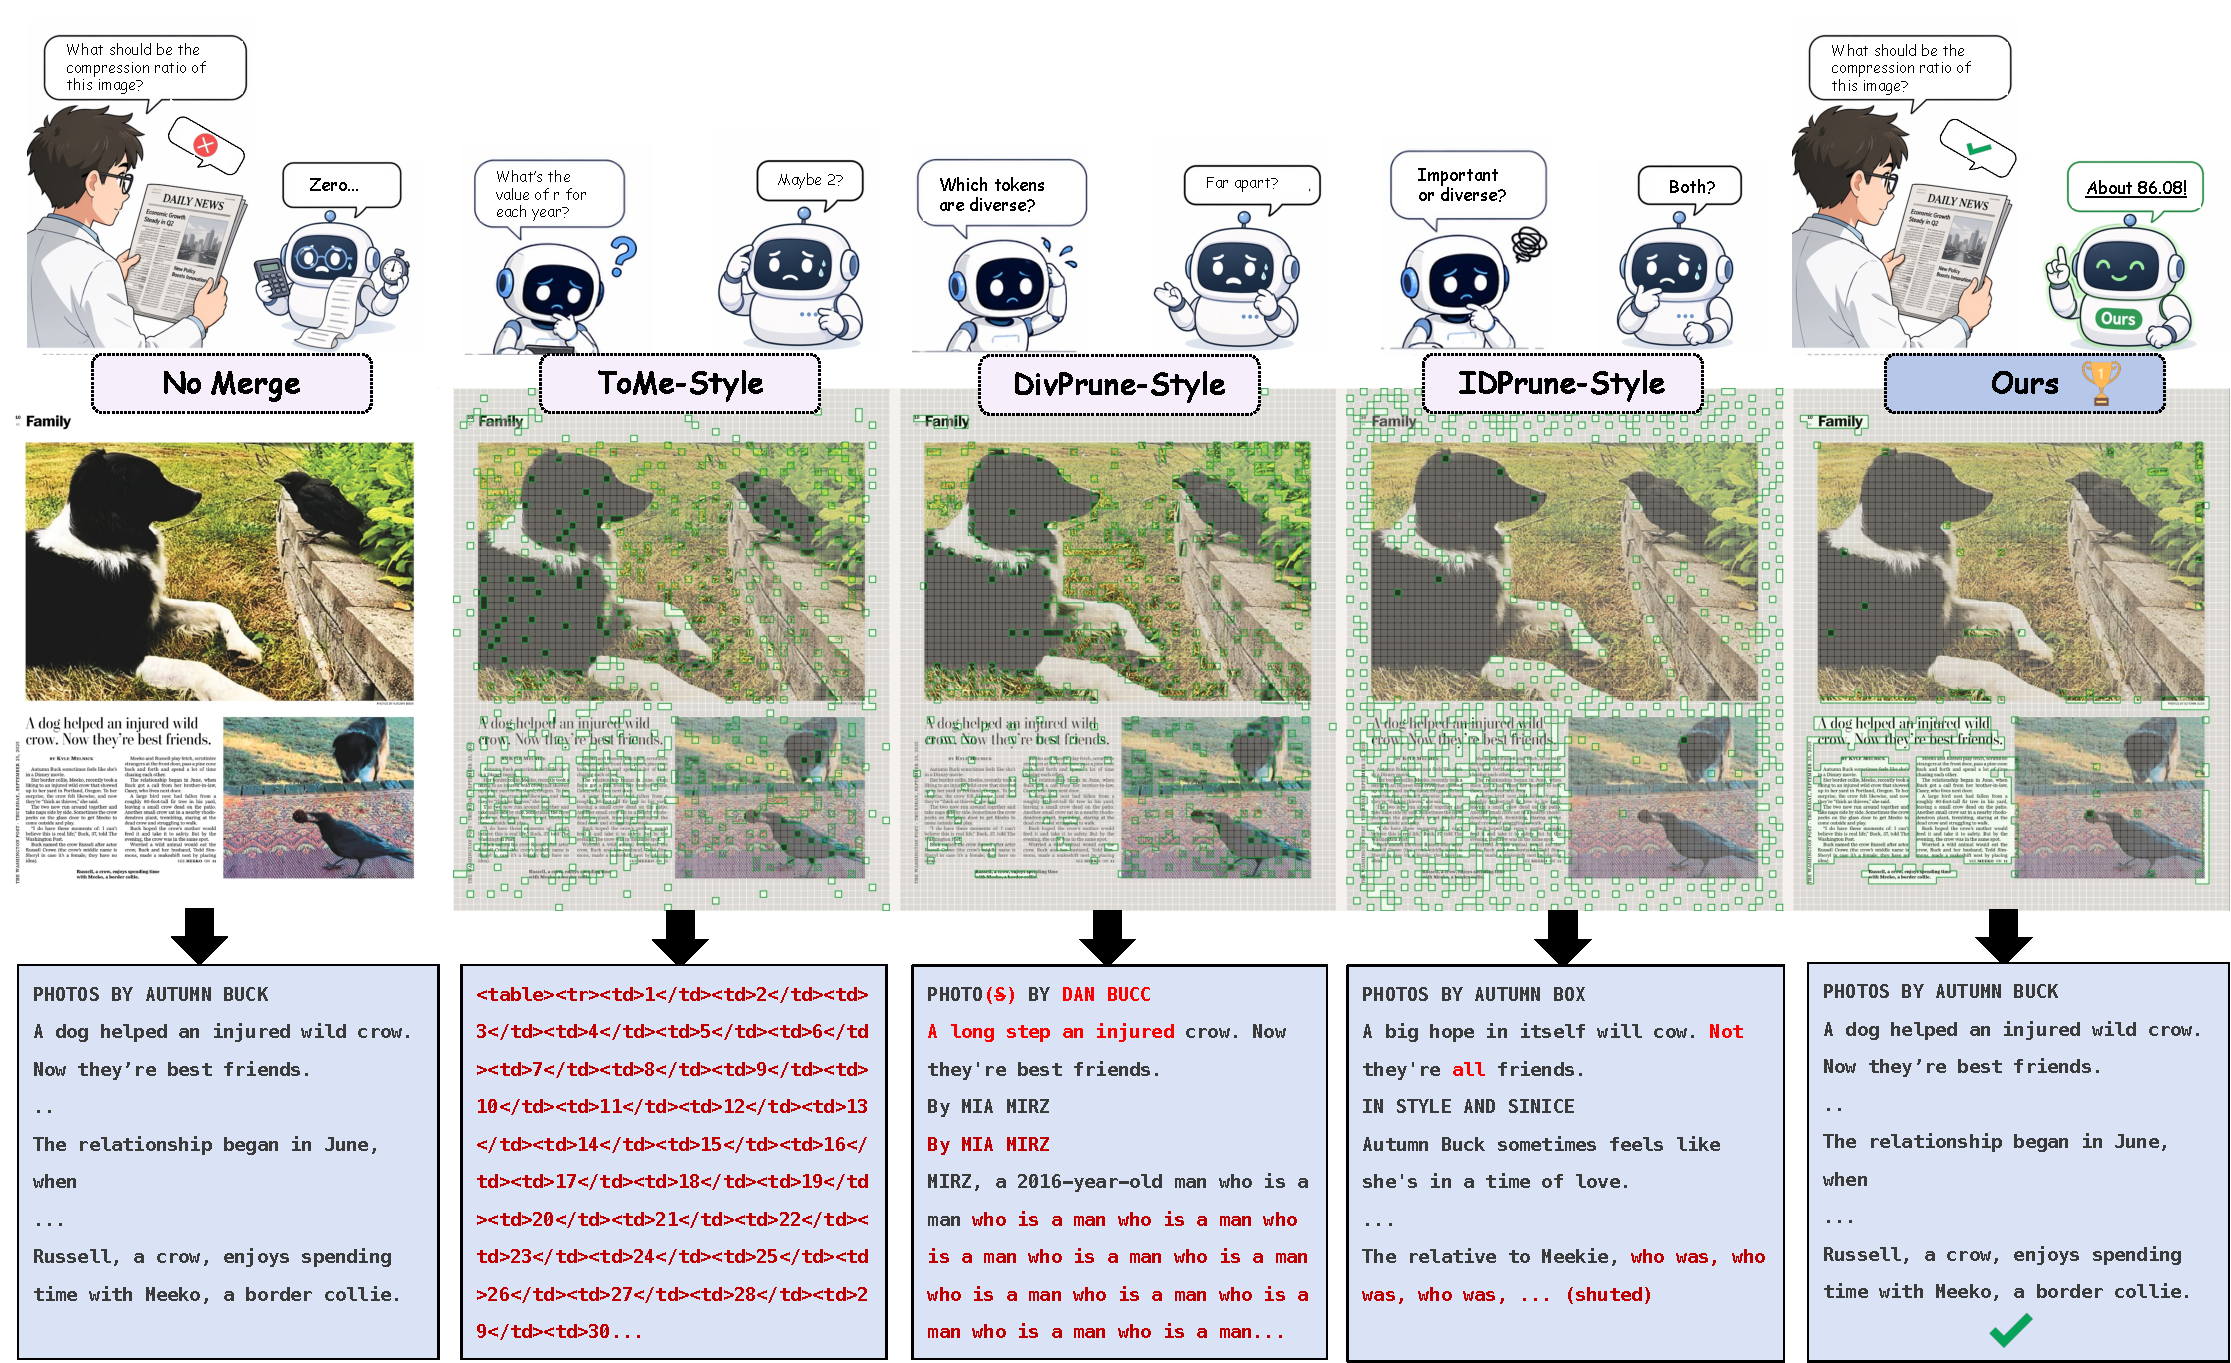
\includegraphics[width=\linewidth]{figures/final/compare_other_method.pdf}
\caption{Qualitative comparison of compression rules under a matched token budget on
PaddleOCR-VL-1.6. Top: retained-token maps for No~Merge, ToMe-/DivPrune-/IDPrune-style,
and \ours{}. Bottom: the corresponding Markdown parse. Training-free styles produce
garbled or repeated output, while \ours{} stays faithful to the no-merge reference.}
\label{fig:supp_method_parse}
\end{figure*}

\begin{figure*}[t]
\centering
\includegraphics[width=\linewidth]{figures/final/material/heavy_light_compare.pdf}
\caption{Retained-token maps across compression rules on a graphics-heavy magazine page
(top) and an advertisement page (bottom). Training-free styles retain large background
regions, whereas \ours{} concentrates the token budget on textual and structural content.}
\label{fig:supp_heavy_light}
\end{figure*}
%============================================================
% D. More Benchmark Results
%============================================================
\section{More Benchmark Results}
\label{sec:supp_benchmark}

The main text reports the average token-compression rate per
document category. \ours{} sustains high, content-adaptive compression across all scenarios. On the
in-the-wild \textbf{Real5} split, it remains robust to real capture degradations: it filters
environmental shadows and background artifacts to lock onto core textual tokens, yielding large
gains over the fixed reference bound on \textit{Scanning} (71.4\%), \textit{Warping} (78.4\%),
\textit{Screen-Photography} (78.1\%), \textit{Illumination} (75.6\%), and \textit{Skew} (76.1\%).
The consistently high compression under these degradations shows that the K-norm density signal is
driven by textual content rather than by clean digital rendering, so the method transfers from
clean layouts to noisy real-world captures without category-specific tuning.
% TODO(PureBench): 若有 PureBench 实验，补一句真实数字；否则保持删除状态。

%============================================================
% E. Inference Efficiency Across Hardware
%============================================================
\section{Inference Efficiency on 8$\times$H800}
\label{sec:supp_hardware}

We report end-to-end inference latency on $8\times$H800 GPUs in
Table~\ref{tab:hardware}, comparing the uncompressed full-image pass with \ours{} on the
PaddleOCR-VL-1.6 host. Because the merge is decided inside the encoder and is independent
of the serving stack, parsing quality is unchanged; the benefit is that far fewer visual
tokens reach the later ViT blocks and the LLM prefill. We separate the ViT-encoder and
LLM-prefill latency (the two stages that shrink with the retained-token count) from the
decode latency, which is bounded by output length and therefore largely unaffected.

\begin{table}[t]
\centering
\fontsize{7.6}{9}\selectfont
\setlength{\tabcolsep}{4pt}
\begin{tabular*}{\columnwidth}{@{\extracolsep{\fill}}l c c c c@{}}
\toprule
\textbf{Setting} & \textbf{Tokens} &
\shortstack{\textbf{Encoder}\\(ms)$\downarrow$} &
\shortstack{\textbf{Prefill}\\(ms)$\downarrow$} &
\shortstack{\textbf{End-to-end}\\(ms)$\downarrow$} \\
\midrule
% TODO: 填 8xH800 实测 latency（token 数为已知真实值）
E2E (no merge) & 4954 & -- & -- & -- \\
\ours{} (best) & 1434 & -- & -- & -- \\
\bottomrule
\end{tabular*}
\caption{Inference latency of \ours{} on $8\times$H800 (PaddleOCR-VL-1.6 host). Retained
visual-token counts are exact; per-stage latency is measured under a fixed input
resolution and batch size. \ours{} lowers encoder and prefill latency by shortening the
visual sequence, while decode latency is bounded by output length and largely unchanged.}
\label{tab:hardware}
\end{table}

%============================================================
% F. Qualitative Visualizations
%============================================================
\section{Qualitative Visualizations}
\label{sec:supp_vis}

We provide extensive qualitative examples of \ours{} across challenging document categories. For
each example we show the visual-token reconstruction after compression alongside the reconstructed
Markdown parse, so both the retained-token layout and the downstream parse can be inspected
together. Across all cases, \ours{} aggressively filters redundant background patches (e.g., blank
regions in scanned pages) while preserving high fidelity in dense semantic areas and fine layout
boundaries, confirming that token reduction does not drop vital layout cues.

Figures~\ref{fig:overview1}--\ref{fig:overview6} span academic papers and textbooks, daily
newspapers, research reports and slides, and structurally irregular handwritten notes and vertical
layouts.

\clearpage
\newpage
\onecolumn

\begin{figure}[t]
\centering
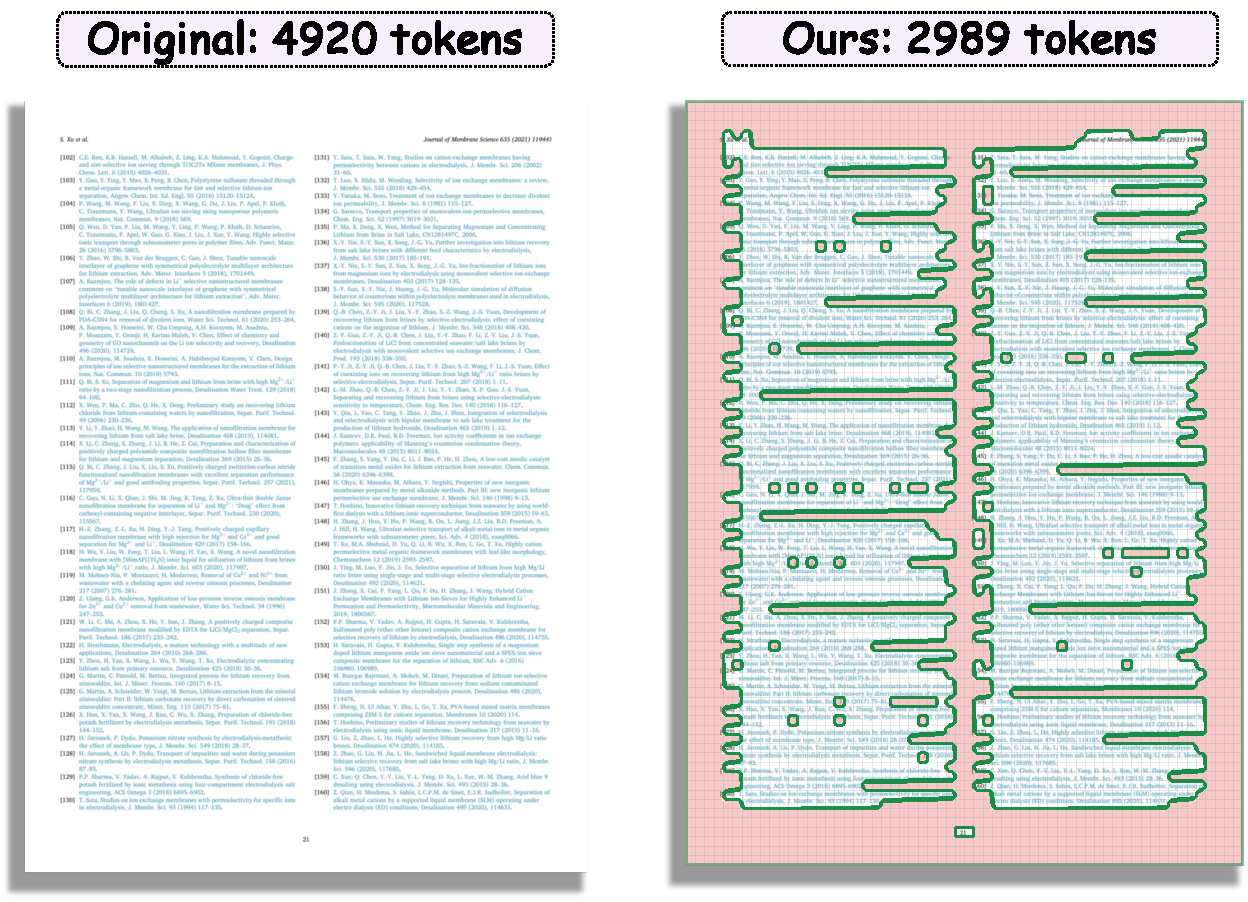
\includegraphics[width=\linewidth]{figures/final/material/paper_1.pdf}
\caption{\centering Visual token reconstruction and Markdown output for compressed
\textbf{Academic Papers} and \textbf{Textbooks}.}
\label{fig:overview1}
\end{figure}

\clearpage
\newpage
\begin{figure}[t]
\centering
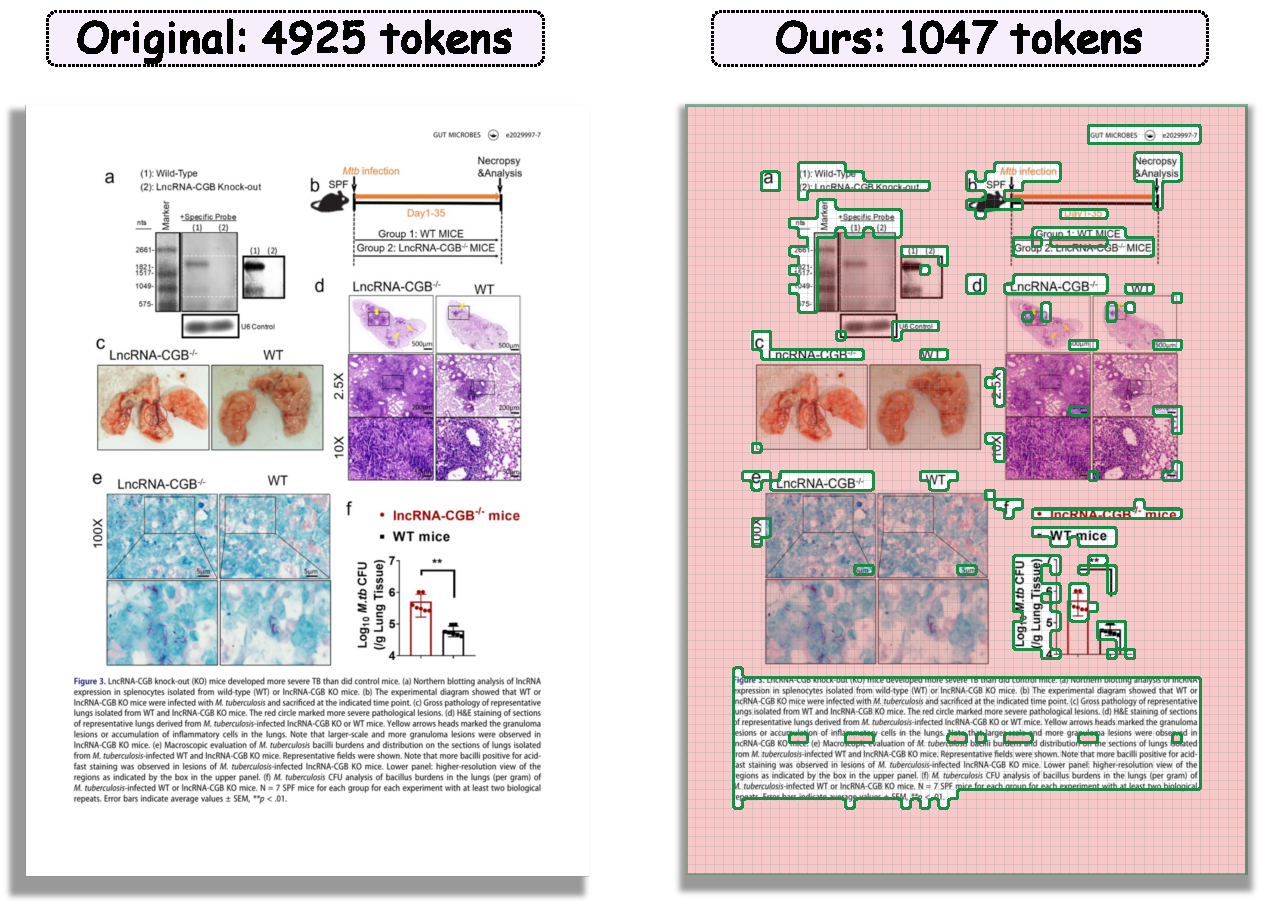
\includegraphics[width=\linewidth]{figures/final/material/paper_2.pdf}
\caption{\centering Visual token reconstruction and Markdown output for compressed
\textbf{Academic Papers} and \textbf{Textbooks}.}
\label{fig:overview2}
\end{figure}

\clearpage
\newpage
\begin{figure}[t]
\centering
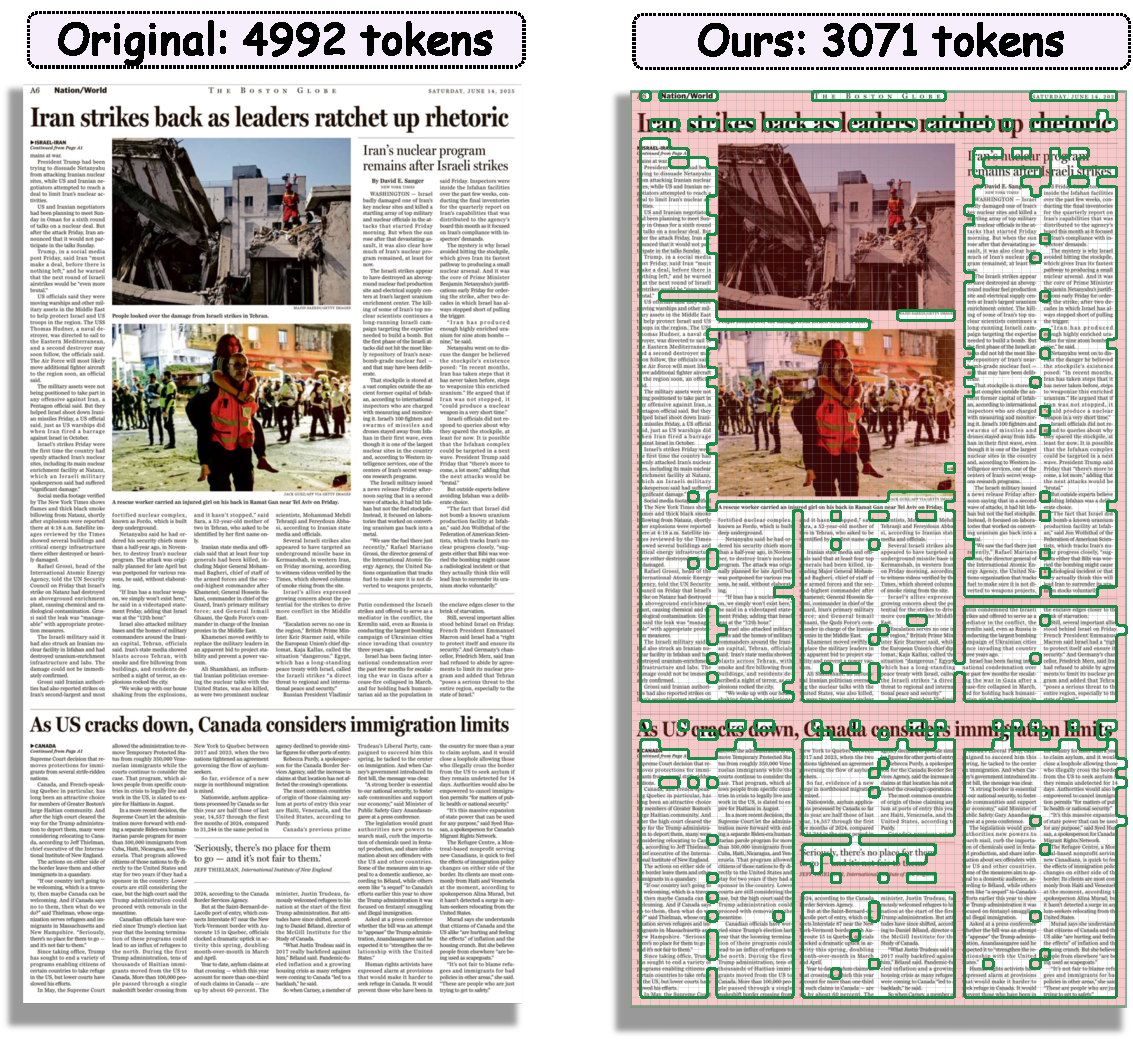
\includegraphics[width=\linewidth]{figures/final/material/news_1.pdf}
\caption{\centering Visual token reconstruction and Markdown output for compressed
\textbf{Daily Newspapers}.}
\label{fig:overview3}
\end{figure}

\clearpage
\newpage
\begin{figure}[t]
\centering
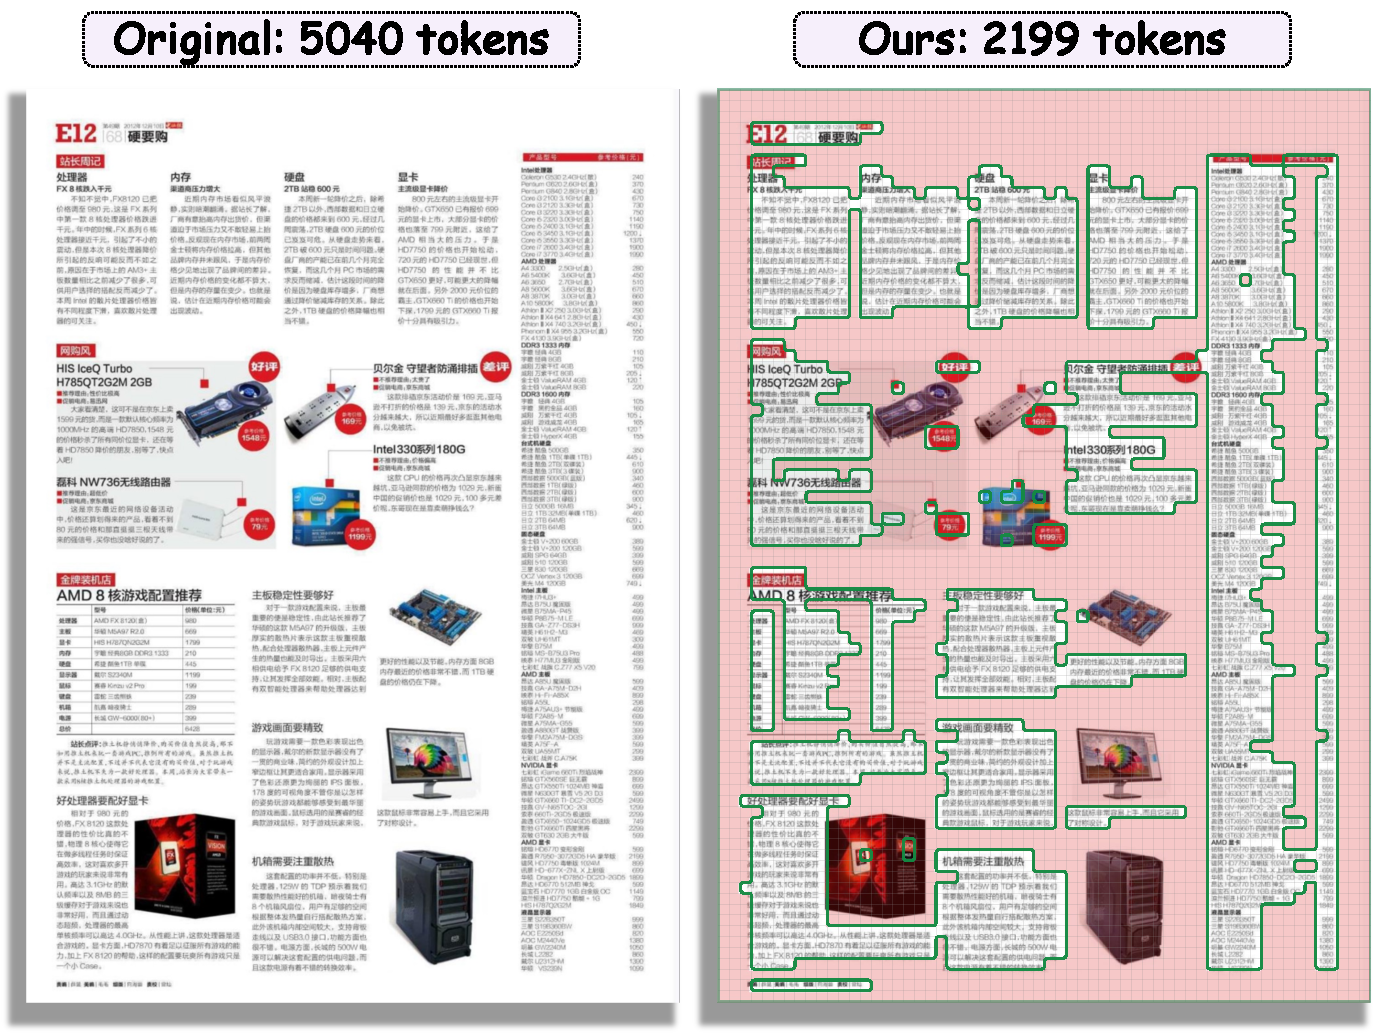
\includegraphics[width=\linewidth]{figures/final/material/news_2.pdf}
\caption{\centering Visual token reconstruction and Markdown output for compressed
\textbf{Daily Newspapers}.}
\label{fig:overview4}
\end{figure}

\clearpage
\newpage
\begin{figure}[t]
\centering
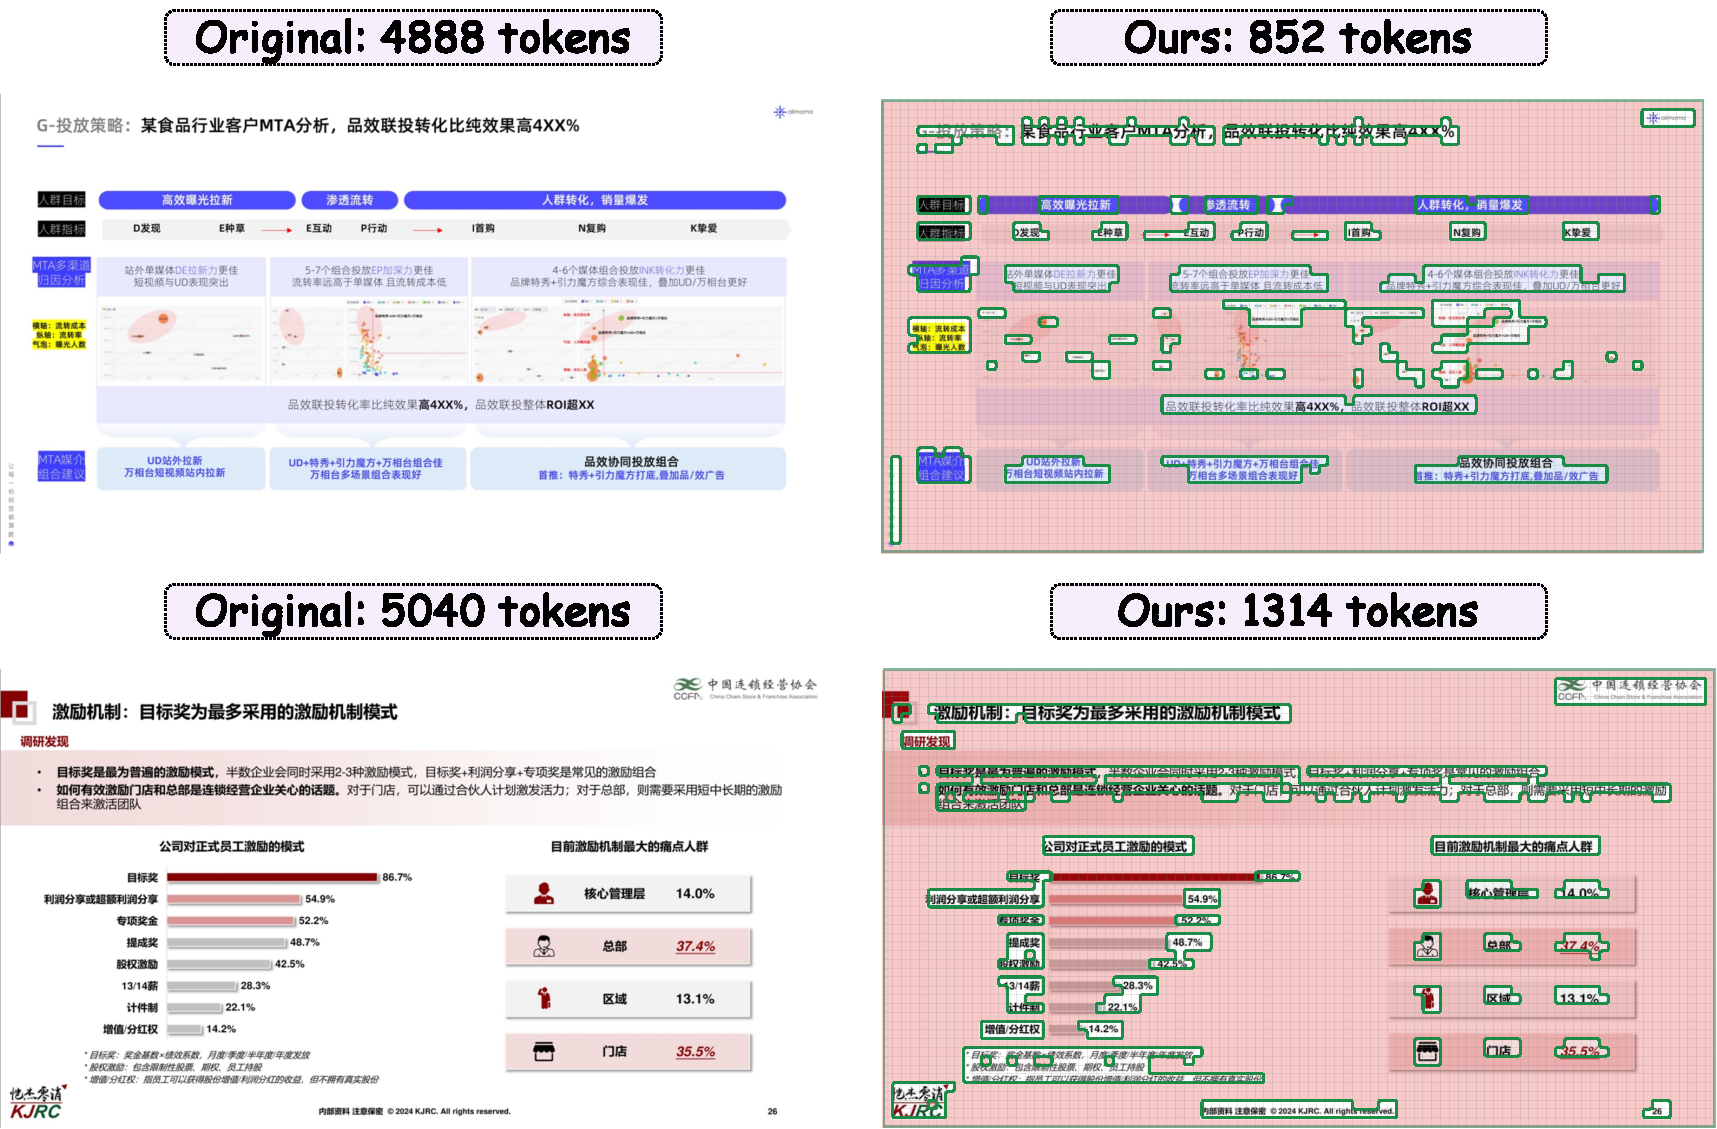
\includegraphics[width=\linewidth]{figures/final/material/ppt_1.pdf}
\caption{\centering Visual token reconstruction and Markdown output for highly formatted documents
including Research Reports and Slides under compression.}
\label{fig:overview5}
\end{figure}

\clearpage
\newpage
\begin{figure}[t]
\centering
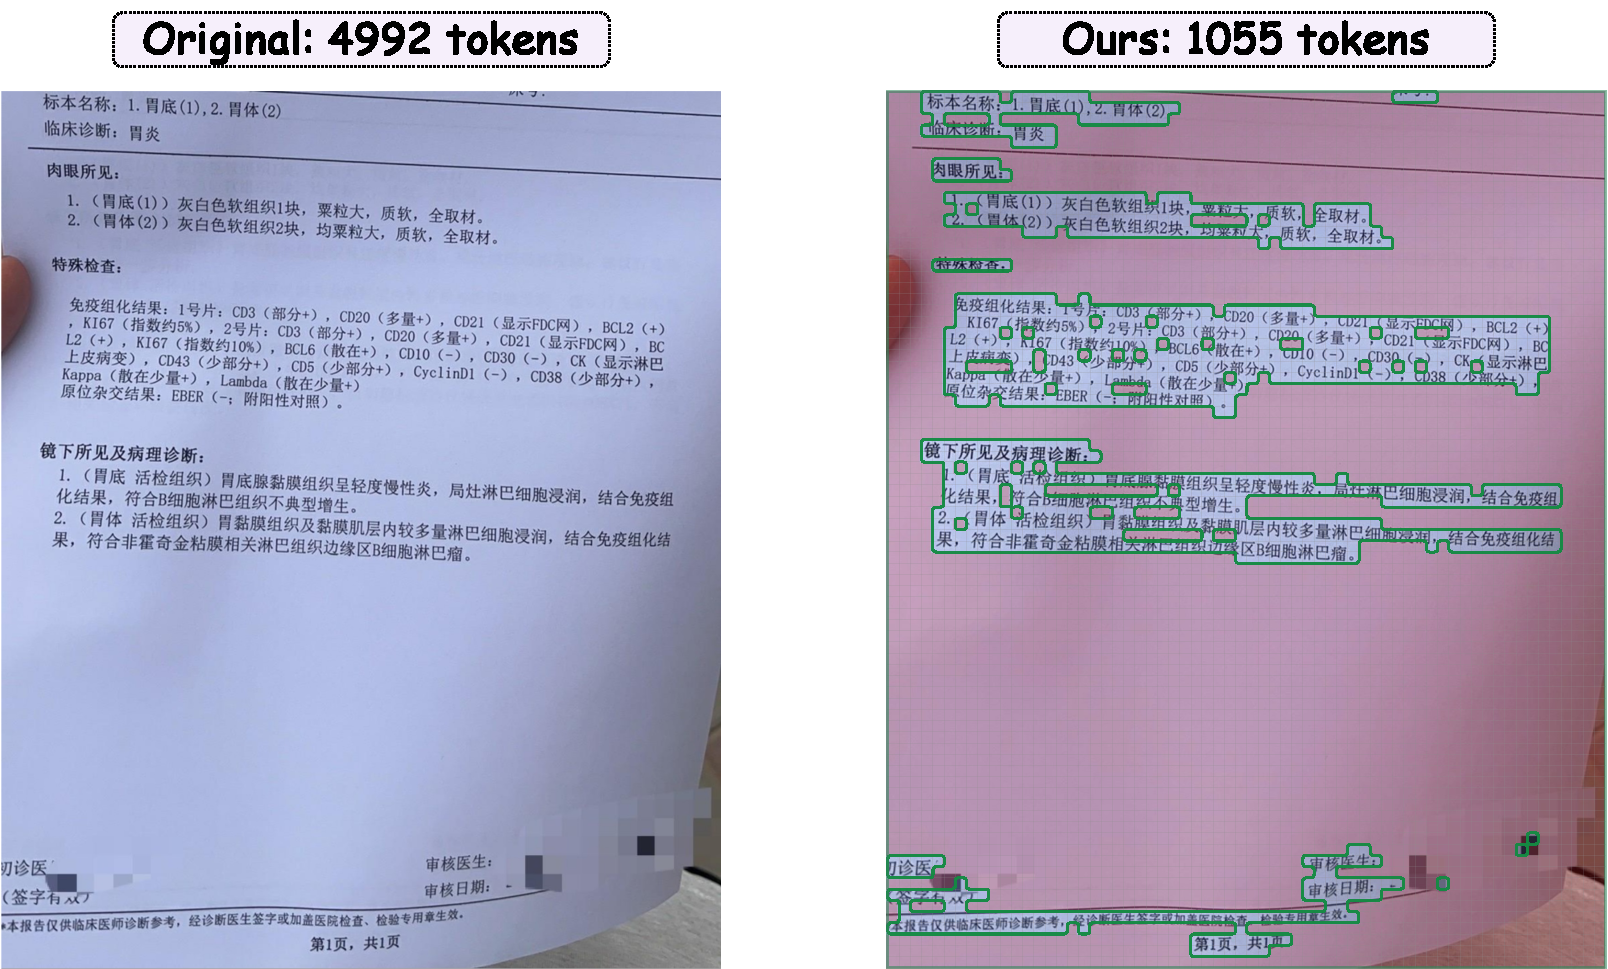
\includegraphics[width=\linewidth]{figures/final/material/real_1.pdf}
\caption{\centering Visual token reconstruction and Markdown output for structurally irregular
\textbf{Handwritten Notes} and vertical text layouts.}
\label{fig:overview6}
\end{figure}

\end{CJK}
\end{document}
